\chapter{Einleitung}

\section{Motivation}
Die Idee der vorliegenden Arbeit entstand mit der Abteilung CSC FI OES LMS der Infineon Technologies AG. 
In der Abteilung arbeite ich schon seit circa zwei Jahren als Werkstudent, an Themen wie Web und Mobile-App-Entwicklung unter meinem Betreuer Florian Saller und meinem Zweibetreuer Fabian Vilsmeier.
Zusammen mit diesen, und meinem Auftraggeber Thomas Gombocz, der bei Infineon in München sitzt, habe ich mein Thema des automatisierten technischen Feasibility Checks für die Durchführung von Qualifikationen neuer Halbleiter-Produkte ausgearbeitet.


\section{Zielsetzung der Arbeit}
In dieser Bachelorarbeit wird ein sogenannter technischer Feasibility Check, zu deutsch Machbarkeitsstudie, geplant und umgesetzt. Dieser ist Bestandteil einer größeren internen Software-Applikation namens \ac{REALIS}(diese wird genauer beschrieben in Kapitel~\ref{Sec:REALIS}), welches
im Zuge einer Migration \todo{was für eine Migration?} von einer Windows-Applikation zu einer Web-Applikation zusätzlich verbessert und modernisiert werden soll. Dabei ist der Feasibility Check ein neues Feature, dass zuvor manuell von Anwendern durchgeführt wurde, und nun automatisiert werden soll.

Der Feasibility Check ist eine Backend-Logik, geschrieben in der Programmiersprache C\#, die durch einen einfachen HTTP-Aufruf auf dem Frontend, einer Website, gestartet wird. Dabei greift der Algorithmus auf Daten in der Datenbank zu und liefert ein Ergebnis zurück.

Neben der Backend-Entwicklung werden in dieser Arbeit auch ein erweitertes Datenbankmodell konzipiert und eine erste Schnittstelle mit Angular auf der Website programmiert. \todo{was noch alles?}

\section{Software-Entwicklungsprozess}
Software-Entwicklungsprozesse werden durch sogenannte Vorgehensmodelle beschrieben. Das Ziel solcher Modelle ist es, eine Hilfestellung bei der Organisation von Software-Entwicklungsprojekten zu geben und die Menge aller dabei anfallenden Aktivitäten in klare und verbindliche Arbeitsschritte aufzuteilen. 

Für dieses Projekt wird das Prototyping-Modell eingesetzt. In diesem Ansatz werden schrittweise Prototypen basierend auf den aktuellen Anforderungen entwickelt. Das daraufhin eingeholte Feedback von Auftraggebern oder Endanwendern ermöglicht eine kontinuierliche Verfeinerung der Anforderungen und eine schrittweise Verbesserung des Prototyps. Die Stadien dieses Modells werden in Abbildung~\ref{fig:Prototyping-Modell} nochmal verdeutlicht \cite{senarath2021waterfall}.

\begin{figure}[h!]
    \centering
    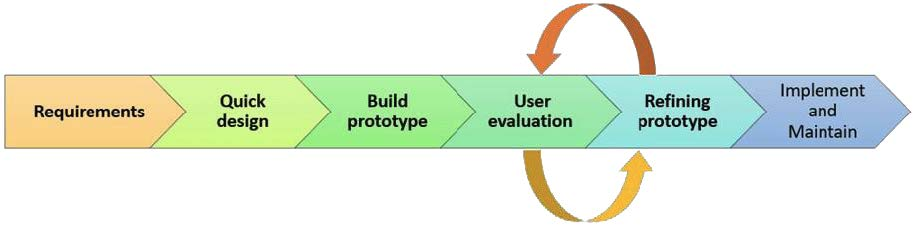
\includegraphics[]{bilder/Prototyping_Stages.jpg}
    \caption{Prototyping-Modell Stadien}
    \label{fig:Prototyping-Modell}
\end{figure}

Das Prototyping-Modell wurde eingesetzt, da die Anforderungen des technischen Feasibility Checks zu Beginn noch nicht eindeutig definiert waren und erst im Laufe der Entwicklung bestimmte Aspekte geklärt werden konnten. Zudem förderte dieser Ansatz den regelmäßigen Austausch zwischen mir als Entwickler und den Auftraggebern.

\section{Aufbau der Arbeit}
Die Bachelorarbeit ist so strukturiert, dass nach diesem einleitenden Kapitel in Abschnitt \ref{Chap:TheoretischeGrundlagen} zuallererst, die wichtigsten theoretischen Grundlagen geklärt werden. 
Hierbei wird kurz Infineon und die Halbleitertechnologie erläutert, woraufhin auf die Software-Applikation \ac{REALIS} eingegangen wird und anschließend kurz erklärt wird, was der englische Titel "Feasibility Check" überhaupt meint. Auch wird noch auf die in der Bachelorarbeit verwendeten Programmiersprachen bzw. Software-Anwendungen und deren Anwendung eingegangen.

Daraufhin werden im Kapitel \nameref{Chap:Anforderungen} die technischen und funktionalen Anforderungen beschrieben, die durch das Prototyping-Modell schrittweise verbessert und bei Bedarf erweitert wurden. Zusätzlich wird eine kurze Stakeholderanalyse durchgeführt.

...

